\section{Core}

The core of Brel consists of filings, facts, components and QNames, where each element is represented by one or more classes.
In essence, each filing consists of a set of facts and components. 
QNames are used all across Brel, which is why they are considered part of the core.
The following UML diagram shows the core of Brel.

\begin{figure}[H]
    \centering
    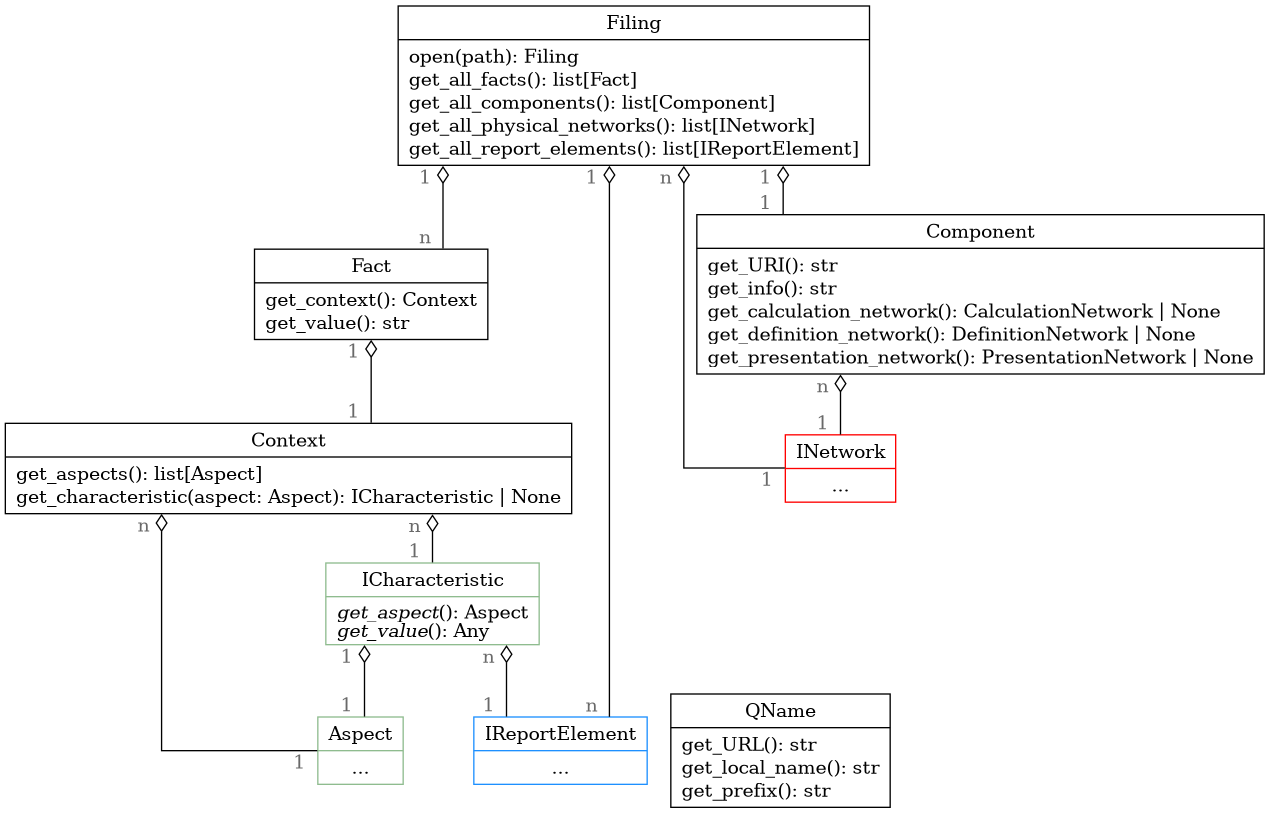
\includegraphics[width=\textwidth]{images/brel_core_classes.png}
    \caption{UML diagram of the core of Brel}
    \label{fig:brel_core_classes}
\end{figure}

\subsection{Filing}
\label{subsec:filing}

Starting with the \texttt{Filing} class, it represents a single XBRL filing.
Obviously, it needs a method for loading a filing from a file, directory, or URL.
The \texttt{Filing.open} covers all of these cases. 
It takes a single argument, which can be a file path, directory path or URL.
The method will automatically detect the type of the argument and load the filing accordingly.
It will also reject any invalid arguments.

The next two methods are \texttt{Filing.get\_all\_facts} and \texttt{Filing.get\_all\_components},
which return all facts and components of the filing, respectively.
Both the facts and components are returned as a list of \texttt{Fact} and \texttt{Component} objects.
The order of the facts and components is not guaranteed.
Brel does provide helper methods for getting specific facts and components,
but their functionality can be easily implemented using the \texttt{get\_all\_facts} and \texttt{get\_all\_components} methods.

There exist some networks that are not part of any Component, specifically \texttt{physical\ networks}.
These networks cannot be accessed indirectly through Components, 
which is why the \texttt{Filing} class also provides a method for getting all physical networks.
This method is aptly named \texttt{Filing.get\_all\_physical\_networks}.

Similar to networks that are not part of any Component, 
there are also report elements that are not part of any network or fact.
The method \texttt{Filing.get\_all\_report\_elements} returns all report elements of the filing,
including both report elements that are referenced by facts or networks and those that are not.

The two most important classes associated with a filing are \texttt{Fact} and \texttt{Component}.
Both classes encompass two different core aspects of XBRL.
All classes belonging to facts are covered by the Open Information Model (OIM)\cite{oim}.
Their design will therefore answer research question \ref{itm:research_question_1}.
Classes belonging to components mostly involve topics that are not covered by the OIM.
Consequently, their design will answer research question \ref{itm:research_question_2}.

The subsequent sections will first describe the \texttt{QName} class,
since it is used by numerous other classes.
The next few sections will cover the \texttt{Fact} class and all of its associated classes.
Finally, the last subsections are dedicated to the \texttt{Component} class and its associated classes.

\subsection{QName}
\label{subsec:qname}

The \texttt{QName} class represents a qualified name, which is a combination of a namespace and a local name.
It is the only remnant of the underlying XML structure of XBRL in the Brel API.
Since it already provides an elegant way of identifying elements across different namespaces,
We chose to keep it in the API.

As described in chapter \ref{chapter:xbrl}, a QName is a combination of a namespace URL, a prefix and a local name.
Naturally, the \texttt{QName} class provides methods for accessing all three of these components.
These methods are fittingly named \texttt{QName.get\_URL}, \texttt{QName.get\_prefix} and \texttt{QName.get\_local\_name}.

\subsection{Fact}
\label{subsec:fact}

The \texttt{Fact} class represents, as the name suggests, a single XBRL fact.
When boiled down to its core, a fact consists of a value and a set of characteristics that describe what the value represents.
The value of a fact is represented by the \texttt{Fact.get\_value} method, which returns the value as a string.
The characteristics of a fact are represented by the \texttt{Fact.get\_context} method.
A context is a set of characteristics that describe the fact.
In other terms, each fact occupies a position in a multi-dimensional space, where each characteristic represents a point along one dimension.

One design decision that seems questionable at first is the \texttt{Fact.get\_value} method, which returns the value as a string.
Not all values in XBRL are strings.
Some are integers, decimals, dates, etc.
The reason for this design decision is that Facts have a unit characteristic, which determines the type of the value.
% The unit of a fact determines the type of the value.
Therefore, units in XBRL are represented as a dimension of the fact's context.
% Therefore, the type of the value can be determined by looking at the unit of the fact.
Since all values that XBRL facts can take are representable as strings, the \texttt{Fact.get\_value} method returns the value as a string,
since it is the most general representation of the value.

Brel does however provide helper methods for converting the value into the type that most appropriately represents the value.
The helper method checks the unit of the fact and converts the value accordingly.

\subsection{Context}

Contexts, as described in section \ref{subsec:fact}, are sets of characteristics what a fact represents.
The \texttt{Context} class represents a single context.
Each fact has its own context and each context belongs to exactly one fact.
\footnote{There might be multiple contexts that have identical characteristics, but they are still represented as separate objects.}
Contexts provide two methods for accessing their characteristics.
The \texttt{Context.get\_aspects} method returns a list of all aspects for which the context has a characteristic.
The \texttt{Context.get\_characteristic} method returns the characteristic of the context for a given aspect.
If the context does not have a characteristic for the given aspect, the method returns \texttt{None}.

To reiterate, a characteristic represents a point along a dimension single dimension.
Multiple characteristics can be combined to form a point in a multi-dimensional space.

One such point might be "Foo Inc.'s net income for the year 2020 in USD".\label{point:foo_net_income}
Another point might be "Bar Corp.'s net income for the year 2021 in CHF".
Both points point to values in a four-dimensional hypercube.
\footnote{In these examples, the four dimensions are entity, period, unit and concept.}

\subsection{Aspect and Characteristics}

Aspects describe the dimensions along which characteristics are positioned.
Their API is described in section \ref{subsec:characteristics}, which will be covered in a later portion of this chapter.

\subsection{Report Elements}

Report elements are the building blocks of XBRL filings.
Probably the most important report element is the concept, initially explained in section \ref{sec:concepts}.
In figure \ref{fig:brel_core_classes}, the interface \texttt{IReportElement} represents all report elements, not just concepts.

Obviously, some characteristics use report elements to describe the position of a fact along a dimension.
Take the previous example \ref{point:foo_net_income} for instance.
One of the characteristics uses the concept "net income" to describe the position of the fact along the concept dimension.
In this case, the characteristic is uses the concept "net income". 

Since there are multiple types of report elements, the \texttt{IReportElement} interface provides a method for getting the type of the report element.
Report elements have their own dedicated section \ref{sec:report_elements}, which will be covered in a later portion of this chapter.

\subsection{Component}

Moving on to the other side of figure \ref{fig:brel_core_classes}, the \texttt{Component} class represents the chapters of a filing.
Components are the first class not by the OIM.

Each component consists of a number of networks and an identifier.
A component can have at most one network of each type.
The available network types are calculation-, presentation- and definition networks.
Additionally, a component can have an optional human-readable description of what the component represents.

The \texttt{Component.get\_calculation\_network}, \texttt{Component.get\_presentation\_network} and \texttt{Component.get\_definition\_network} methods
return the calculation, presentation and definition network of the component, respectively.
Each of these methods can return \texttt{None}, if the component does not have a network of the requested type.

The \texttt{Component.get\_uri} method returns the identifier of the component,
which is a URI that uniquely identifies the component within the filing.

The \texttt{Component.get\_info} method returns the human-readable description of the component, if it exists.
If the component does not have a description, the method returns an empty string.

The networks that are part of a component are represented by the \texttt{Network} class.
Networks will be covered in the second half of this chapter.
The first half focuses on OIM concepts, while the second half focuses on non-OIM concepts.
